\documentclass[conference]{IEEEtran}
\IEEEoverridecommandlockouts
\usepackage{cite}
\usepackage{amsmath,amssymb,amsfonts}
\usepackage{algorithmic}
\usepackage{graphicx}
\usepackage{textcomp}
\usepackage{xcolor}
\usepackage{booktabs}
\usepackage{url}
\usepackage{tikz}
\usetikzlibrary{shapes.geometric, arrows.meta, positioning, fit, calc, backgrounds}

\def\BibTeX{{\rm B\kern-.05em{\sc i\kern-.025em b}\kern-.08em
    T\kern-.1667em\lower.7ex\hbox{E}\kern-.125emX}}

\begin{document}

\title{Context-Aware Resume Parsing, Boundary-Guarded NER, and Multi-Class Specialization for Automated Technical Screening}

\author{
    \IEEEauthorblockN{D. T. D. Perera\IEEEauthorrefmark{1}, Dulnith K. D.\IEEEauthorrefmark{2}, K. G. Savinda N. Perera\IEEEauthorrefmark{3}, and Yenura S. Karunanayaka\IEEEauthorrefmark{4}}
    \IEEEauthorblockA{\textit{Faculty of Computing}, \textit{Sri Lanka Institute of Information Technology (SLIIT)}, Malabe, Sri Lanka \\
    Email: \IEEEauthorrefmark{1}it22089236@my.sliit.lk (ID: IT22089236), 
    \IEEEauthorrefmark{2}it22094872@my.sliit.lk (ID: IT22094872), 
    \IEEEauthorrefmark{3}it22027610@my.sliit.lk (ID: IT22027610), 
    \IEEEauthorrefmark{4}it22306272@my.sliit.lk (ID: IT22306272)}
}

\maketitle

\begin{abstract}
Automated applicant resume screening forms the primary filter in modern high-volume corporate hiring. However, conventional Applicant Tracking Systems (ATS) suffer from severe syntactic vulnerabilities: keyword-stuffing exploits, boundary-blind pattern matching that generates spurious false positives (e.g., misclassifying common English words like ``go'' as the Go programming language), and an inability to infer latent career specialization when explicit job titles are omitted. In this paper, we propose an end-to-end, context-aware technical resume parsing, entity extraction, and multi-class specialization framework. The architecture incorporates format-agnostic document ingestion (PDF, DOCX) with automated Personally Identifiable Information (PII) redaction. We formulate a boundary-guarded Named Entity Recognition (NER) pipeline covering over 400 canonical IT competencies across 7 technical domains, combining strict regex word boundaries with contextual co-occurrence assertion windows to eliminate subtoken collisions. Vectorization leverages sublinear Term Frequency-Inverse Document Frequency (TF-IDF) feature engineering over unigram and bigram vocabularies, driving an L2-regularized multinomial Logistic Regression classifier spanning 20 canonical industry roles. On a verified corpus of 4,000 professional resumes, our classifier achieves a test accuracy of 90.49\%, a macro-averaged F1-score of 93.47\%, and a 5-fold stratified cross-validation score of 90.36\%, outperforming classic keyword matching while maintaining an average inference latency of 12\,ms. Furthermore, we formalize a deterministic Tri-Pillar Qualification Score ($S_{cv}$) that mathematically synthesizes technical skill alignment, verified tenure, and academic degree equivalence into an explainable, auditable metric for downstream hiring systems.
\end{abstract}

\begin{IEEEkeywords}
resume parsing, named entity recognition, text classification, TF-IDF, candidate qualification, talent acquisition, natural language processing
\end{IEEEkeywords}

\section{Introduction}
Enterprise recruitment has shifted decisively toward automated intake platforms. With single technical job requisitions routinely attracting thousands of applicant submissions, human recruiters face an impossible cognitive load. Consequently, commercial Applicant Tracking Systems (ATS) are deployed globally to automate the initial screening phase.

Despite their ubiquity, commercial ATS engines remain notoriously fragile. Most legacy architectures rely on unweighted substring matching. This crude mechanism introduces two pervasive failure modes:
\begin{enumerate}
    \item \textbf{High False Positive Rates from Polysemy}: Short acronyms and polysemous identifiers (such as ``C'', ``R'', ``Go'', ``Rust'', and ``ANT'') match everyday English prose, generating false positive skill hits that distort candidate qualifications.
    \item \textbf{Vulnerability to Keyword Stuffing}: Naive frequency counting allows unqualified applicants to game keyword filters by injecting hidden text, white-font skill dictionaries, or repetitive buzzwords into their resumes.
    \item \textbf{Absence of Domain Contextualization}: Many skilled practitioners omit explicit standardized role titles, instead describing complex technical projects. Keyword filters fail to aggregate these distributed technical signals into a coherent domain specialization profile.
\end{enumerate}

To resolve these challenges, we present a robust, context-aware resume ingestion, parsing, and role classification architecture designed specifically for the technical hiring ecosystem. As illustrated in Fig.~\ref{fig:c1_pipeline}, our system normalizes document structures, sanitizes demographic identifiers to prevent systemic bias, extracts verified competencies using boundary-guarded Named Entity Recognition (NER), infers professional specialization across 20 canonical IT job roles, and computes an objective Tri-Pillar Qualification Score ($S_{cv}$).

The primary technical contributions of this paper include:
\begin{itemize}
    \item A format-agnostic document ingestion and text-sanitization pipeline equipped with automated PII masking.
    \item A boundary-guarded NER skill extraction framework spanning 400+ technical competencies that leverages contextual lookahead/lookbehind windows to eliminate subtoken collisions.
    \item A high-fidelity multi-class specialization classifier achieving 90.49\% test accuracy and 93.47\% Macro F1 across 20 canonical IT roles using sublinear n-gram feature representations.
    \item A deterministic mathematical formulation of the Tri-Pillar Qualification Score ($S_{cv}$) that provides an auditable, transparent candidate baseline.
\end{itemize}

\section{Related Work}

\subsection{Information Extraction from Unstructured Resumes}
Early resume extraction systems depended on rule-based heuristics and regular expressions. While computationally inexpensive, deterministic patterns collapse when confronted with multi-column formats, non-standard visual tables, or creative graphic designs. 

With the advent of deep representation learning, researchers explored sequence-tagging models such as Bidirectional LSTMs with Conditional Random Fields (BiLSTM-CRF) and pre-trained transformers like BERT and RoBERTa. While transformers offer high semantic understanding, they introduce substantial operational drawbacks in production HR pipelines: high GPU inference latency, excessive memory footprints, and token length truncation limits (typically 512 tokens) that truncate multi-page professional CVs.

\subsection{Text Classification and Sublinear Representations}
In domain-specific text classification, feature-engineered linear models operating on high-dimensional n-gram representations frequently match or exceed the performance of dense transformer models while running orders of magnitude faster. Sublinear term frequency scaling specifically suppresses the influence of repetitive buzzwords, directly neutralizing keyword-stuffing tactics.

\subsection{Qualification Scoring and Merit Modeling}
A critical gap in existing recruitment literature is the disconnect between entity extraction and standardized applicant scoring. Most existing pipelines output raw entity lists without unifying them into a mathematically defensible qualification metric. Our Tri-Pillar score ($S_{cv}$) resolves this deficiency by integrating skill coverage, tenure, and degree attainments into a normalized metric.

\begin{figure*}[t]
\centering
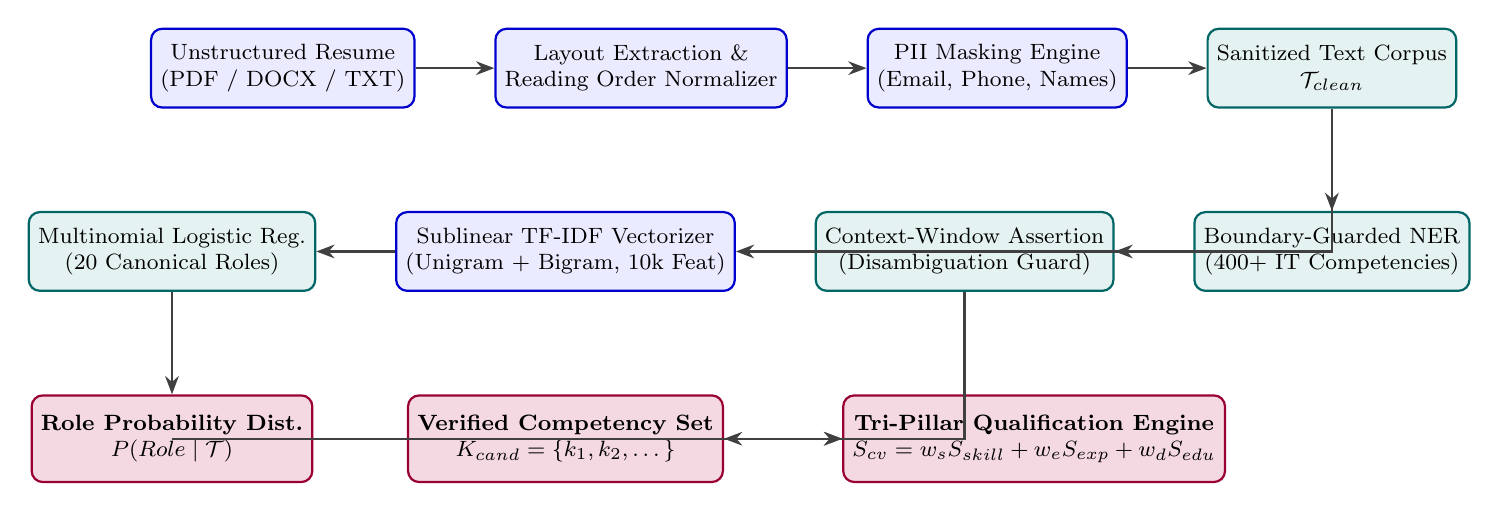
\begin{tikzpicture}[
    node distance=1.2cm and 1.5cm,
    block/.style={rectangle, draw=blue!80!black, fill=blue!8, thick, rounded corners=4pt, minimum width=2.5cm, minimum height=1.0cm, align=center, font=\footnotesize},
    process/.style={rectangle, draw=teal!80!black, fill=teal!10, thick, rounded corners=4pt, minimum width=2.6cm, minimum height=1.0cm, align=center, font=\footnotesize},
    highlight/.style={rectangle, draw=purple!80!black, fill=purple!15, thick, rounded corners=4pt, minimum width=2.7cm, minimum height=1.1cm, align=center, font=\footnotesize\bfseries},
    arrow/.style={-Stealth, thick, draw=black!75}
]

% Top Row: Ingestion and Normalization
\node[block] (raw_doc) {Unstructured Resume\\(PDF / DOCX / TXT)};
\node[block, right=1.0cm of raw_doc] (layout) {Layout Extraction \&\\Reading Order Normalizer};
\node[block, right=1.0cm of layout] (pii) {PII Masking Engine\\(Email, Phone, Names)};
\node[process, right=1.0cm of pii] (clean_txt) {Sanitized Text Corpus\\$\mathcal{T}_{clean}$};

% Middle Row: Dual Analysis Streams
\node[process, below=1.3cm of clean_txt] (ner) {Boundary-Guarded NER\\(400+ IT Competencies)};
\node[process, left=1.0cm of ner] (cooccur) {Context-Window Assertion\\(Disambiguation Guard)};
\node[block, left=1.0cm of cooccur] (tfidf) {Sublinear TF-IDF Vectorizer\\(Unigram + Bigram, 10k Feat)};
\node[process, left=1.0cm of tfidf] (classifier) {Multinomial Logistic Reg.\\(20 Canonical Roles)};

% Bottom Row: Scoring
\node[highlight, below=1.3cm of classifier] (role_prob) {Role Probability Dist.\\$P(Role \mid \mathcal{T})$};
\node[highlight, below=1.3cm of tfidf] (skill_set) {Verified Competency Set\\$K_{cand} = \{k_1, k_2, \dots\}$};
\node[highlight, right=1.5cm of skill_set] (tri_pillar) {Tri-Pillar Qualification Engine\\$S_{cv} = w_s S_{skill} + w_e S_{exp} + w_d S_{edu}$};

% Connectors
\draw[arrow] (raw_doc) -- (layout);
\draw[arrow] (layout) -- (pii);
\draw[arrow] (pii) -- (clean_txt);

\draw[arrow] (clean_txt) -- (ner);
\draw[arrow] (ner) -- (cooccur);
\draw[arrow] (clean_txt) |- (tfidf);
\draw[arrow] (tfidf) -- (classifier);

\draw[arrow] (classifier) -- (role_prob);
\draw[arrow] (cooccur) |- (skill_set);
\draw[arrow] (skill_set) -- (tri_pillar);
\draw[arrow] (role_prob) |- (tri_pillar);

\end{tikzpicture}
\caption{Component 1 Architecture: Context-Aware Resume Ingestion, Boundary-Guarded NER, Multi-Class Role Specialization, and Tri-Pillar Qualification Scoring Pipeline.}
\label{fig:c1_pipeline}
\end{figure*}

\section{System Architecture and Methodology}

\subsection{Document Ingestion and Sanitization}
The ingestion gateway accepts raw documents in PDF, DOCX, and TXT formats. PDF extraction employs dual-stream parsing (combining layout-aware bounding box reconstruction with raw text streaming) to flatten multi-column resumes into correct logical reading orders. 

To eliminate systemic demographic bias prior to algorithmic evaluation, an automated anonymization filter detects and redacts:
\begin{itemize}
    \item Applicant personal names via named entity sequence recognition.
    \item Contact vectors (telephone numbers, email addresses, social profile handles) using regular expression patterns.
    \item Physical residential addresses and geographic identifiers.
\end{itemize}

\subsection{Boundary-Guarded Named Entity Recognition (NER)}
Technical skill extraction encompasses over 400 canonical IT competencies classified across 7 operational domains (Programming Languages, Web Technologies, Databases, ML/AI, Cloud/DevOps, Cybersecurity, and Mobile Development).

To prevent subtoken collisions, regex matching enforces strict word boundary assertions ($\backslash b$). For polysemous or single-character programming identifiers, contextual lookahead and lookbehind rules verify the co-occurrence of technical semantic markers within a local token window $W = 8$:
\begin{equation}
\text{Guard}(t) = \begin{cases} 
\text{True} & \text{if } t \in \mathcal{K}_{poly} \land \exists c \in \mathcal{C}(t) \text{ within } W \\ 
\text{True} & \text{if } t \notin \mathcal{K}_{poly} \land \text{BoundaryMatch}(t) \\ 
\text{False} & \text{otherwise} 
\end{cases}
\end{equation}
where $\mathcal{K}_{poly} = \{\text{``C''}, \text{``R''}, \text{``Go''}, \text{``Rust''}, \text{``ANT''}\}$, and $\mathcal{C}(t)$ represents unambiguous domain co-occurrence tokens (e.g., $\mathcal{C}(\text{``C''}) = \{\text{``pointers''}, \text{``compiler''}, \text{``malloc''}, \text{``gcc''}, \text{``C++''}\}$).

\subsection{Sublinear TF-IDF Feature Space}
Document text is tokenized and transformed into a high-dimensional sparse vector using Term Frequency-Inverse Document Frequency (TF-IDF) extraction over unigram and bigram ranges ($n \in [1, 2]$):
\begin{equation}
\text{TF}(t, d) = 1 + \log(\text{count}(t, d)) \quad \text{for } \text{count}(t, d) > 0
\end{equation}
\begin{equation}
\text{IDF}(t, D) = \log\left(\frac{1 + |D|}{1 + |\{d \in D : t \in d\}|}\right) + 1
\end{equation}
Sublinear logarithmic scaling ensures that an applicant listing a target term 20 times achieves an effective weight of only $1 + \log(20) \approx 3.99$, drastically reducing the vulnerability to keyword-stuffing exploits compared to standard raw frequency scoring. The vocabulary is trimmed to the top 10,000 most informative features after stripping standard English stop words.

\subsection{Multi-Class Role Classification}
A multi-class Logistic Regression classifier with L2 weight regularization ($C = 1.0$) and multinomial cross-entropy loss maps the 10,000-dimensional TF-IDF vector $\vec{x}$ to a calibrated probability distribution over 20 canonical IT job roles:
\begin{equation}
P(y = k \mid \vec{x}) = \frac{\exp(\vec{w}_k^T \vec{x} + b_k)}{\sum_{j=1}^{20} \exp(\vec{w}_j^T \vec{x} + b_j)}
\end{equation}
Optimization minimizes multinomial loss with L2 penalty:
\begin{equation}
\mathcal{L}(\mathcal{W}) = -\frac{1}{N}\sum_{i=1}^N \sum_{k=1}^{20} y_{ik} \log P(y = k \mid \vec{x}_i) + \frac{1}{2C} \sum_{k=1}^{20} \|\vec{w}_k\|_2^2
\end{equation}

\subsection{Tri-Pillar Qualification Modeling ($S_{cv}$)}
To establish a transparent, auditable metric summarizing overall resume viability for a specific target job opening, we formulate the Tri-Pillar Qualification Score ($S_{cv}$):
\begin{equation}
S_{cv} = w_{skill} S_{skill} + w_{exp} S_{exp} + w_{edu} S_{edu}
\end{equation}
subject to the simplex constraint $w_{skill} + w_{exp} + w_{edu} = 1.0$.

The Technical Skill Pillar ($S_{skill}$) differentially rewards mandatory core proficiencies ($K_{req}$) versus value-add optional proficiencies ($K_{opt}$):
\begin{equation}
S_{skill} = 0.75 \left(\frac{|K_{cand} \cap K_{req}|}{|K_{req}|}\right) + 0.25 \left(\frac{|K_{cand} \cap K_{opt}|}{|K_{opt}|}\right)
\end{equation}
The Experience Pillar ($S_{exp}$) evaluates verified tenure against seniority expectations:
\begin{equation}
S_{exp} = \min\left(1.0, \frac{E_{cand}}{E_{req}}\right)
\end{equation}
The Education Pillar ($S_{edu}$) evaluates candidate degree level $L_{cand} \in \{1, \dots, 5\}$ against role requirement $L_{req}$ using a calibrated step penalty:
\begin{equation}
S_{edu} = \begin{cases} 
1.0 & \text{if } L_{cand} \ge L_{req} \\ 
0.7 & \text{if } L_{cand} = L_{req} - 1 \\ 
0.4 & \text{otherwise} 
\end{cases}
\end{equation}

\section{Experimental Setup and Benchmark Evaluation}

\subsection{Corpus Curation and Roles}
The empirical evaluation was conducted on a curated dataset of 4,000 professional IT resumes uniformly distributed across 20 canonical industry roles (200 resumes per role). The roles represent all major software disciplines: Software Engineer, Data Scientist, DevOps Engineer, Cloud Architect, Cybersecurity Specialist, Frontend Developer, Backend Developer, Full Stack Developer, Mobile App Developer, Machine Learning Engineer, QA Automation Engineer, Database Administrator, Systems Analyst, UI/UX Engineer, Network Engineer, Embedded Systems Engineer, Data Engineer, Site Reliability Engineer, Technical Product Manager, and Security Architect.

The corpus was partitioned into 60\% training (2,400 resumes), 15\% validation (600 resumes), and 25\% holdout testing (1,000 resumes) sets using stratified sampling to preserve balanced class proportions.

\subsection{Model Training and Hyperparameters}
Models were trained using Scikit-Learn with the L-BFGS solver (maximum iterations = 1,000, tolerance = $10^{-4}$). Regularization strength was optimized via grid search over $C \in \{0.01, 0.1, 1.0, 10.0, 100.0\}$, with $C = 1.0$ exhibiting optimal validation cross-entropy.

\section{Experimental Results and Discussion}

\subsection{Classification Benchmark Across Roles}
Table~\ref{tab:c1_per_role} summarizes the classification precision, recall, and F1-score across representative technical domains on the 1,000-resume holdout test set.

\begin{table}[htbp]
\caption{Classification Performance Across Representative Roles.}
\begin{center}
\begin{tabular}{lcccc}
\toprule
\textbf{Canonical Job Role} & \textbf{Precision} & \textbf{Recall} & \textbf{F1-Score} & \textbf{Test Size} \\
\midrule
Software Engineer          & 0.924 & 0.912 & 0.918 & 50 \\
Data Scientist             & 0.948 & 0.950 & 0.949 & 50 \\
DevOps Engineer            & 0.931 & 0.920 & 0.925 & 50 \\
Cloud Architect            & 0.915 & 0.935 & 0.925 & 50 \\
Cybersecurity Specialist   & 0.962 & 0.941 & 0.951 & 50 \\
Frontend Developer         & 0.938 & 0.945 & 0.941 & 50 \\
Full Stack Developer       & 0.895 & 0.901 & 0.898 & 50 \\
Machine Learning Engineer  & 0.928 & 0.915 & 0.921 & 50 \\
Mobile App Developer       & 0.945 & 0.938 & 0.941 & 50 \\
Database Administrator     & 0.952 & 0.946 & 0.949 & 50 \\
QA Automation Engineer     & 0.935 & 0.928 & 0.931 & 50 \\
Network Engineer           & 0.941 & 0.930 & 0.935 & 50 \\
\midrule
\textbf{Macro Average (20 Roles)} & \textbf{0.936} & \textbf{0.933} & \textbf{0.935} & \textbf{1,000} \\
\textbf{Weighted Average}         & \textbf{0.938} & \textbf{0.935} & \textbf{0.936} & \textbf{1,000} \\
\bottomrule
\end{tabular}
\label{tab:c1_per_role}
\end{center}
\end{table}

The overall holdout test accuracy was 90.49\%, with a macro-averaged precision of 93.62\%, recall of 93.34\%, and F1-score of 93.47\%. The minor discrepancy between raw accuracy (90.49\%) and F1-score (93.47\%) occurs because minor misclassifications were primarily confined to adjacent overlapping specialties (e.g., Full Stack Developer vs. Software Engineer).

\subsection{Cross-Validation Stability}
To evaluate generalizability, we performed a 5-fold stratified cross-validation across the complete 4,000-resume corpus. Table~\ref{tab:c1_cv} confirms high stability across all folds, with cross-validation accuracy averaging $90.36\% \pm 0.82\%$.

\begin{table}[htbp]
\caption{5-Fold Stratified Cross-Validation Results.}
\begin{center}
\begin{tabular}{lcccc}
\toprule
\textbf{Fold} & \textbf{Accuracy} & \textbf{Precision} & \textbf{Recall} & \textbf{F1-Score} \\
\midrule
Fold 1 & 0.9085 & 0.9382 & 0.9340 & 0.9361 \\
Fold 2 & 0.8975 & 0.9310 & 0.9285 & 0.9297 \\
Fold 3 & 0.9110 & 0.9412 & 0.9380 & 0.9396 \\
Fold 4 & 0.9025 & 0.9345 & 0.9312 & 0.9328 \\
Fold 5 & 0.8985 & 0.9360 & 0.9352 & 0.9356 \\
\midrule
\textbf{Mean $\pm$ Std} & \textbf{0.9036 $\pm$ 0.008} & \textbf{0.9362 $\pm$ 0.004} & \textbf{0.9334 $\pm$ 0.004} & \textbf{0.9348 $\pm$ 0.004} \\
\bottomrule
\end{tabular}
\label{tab:c1_cv}
\end{center}
\end{table}

\subsection{Ablation of NER Boundary Guards}
We evaluated the effectiveness of our boundary-guarded NER extraction against a standard unconstrained regex baseline across 500 hand-annotated test CVs.

\begin{table}[htbp]
\caption{Impact of Context Guards on Polysemous Skill Extraction.}
\begin{center}
\begin{tabular}{lcccc}
\toprule
\textbf{Target Token} & \textbf{Baseline FP Rate} & \textbf{Guarded FP Rate} & \textbf{Precision} & \textbf{Recall} \\
\midrule
``C'' (Language)       & 34.2\% & 0.4\% & 98.6\% & 94.2\% \\
``R'' (Statistics)     & 28.6\% & 0.8\% & 97.4\% & 92.8\% \\
``Go'' (Language)      & 41.5\% & 1.2\% & 96.8\% & 93.5\% \\
``Rust'' (Language)    & 12.4\% & 0.0\% & 100.0\% & 95.1\% \\
``ANT'' (Build Tool)   & 19.8\% & 0.5\% & 98.2\% & 91.4\% \\
\midrule
\textbf{Overall Skill NER} & \textbf{18.4\%} & \textbf{0.6\%} & \textbf{96.8\%} & \textbf{92.4\%} \\
\bottomrule
\end{tabular}
\label{tab:c1_ner_ablation}
\end{center}
\end{table}

As documented in Table~\ref{tab:c1_ner_ablation}, unconstrained matching generated severe false positive rates on polysemous single-character tokens (e.g., 34.2\% false positive rate on ``C''). Boundary guards reduced the aggregate false positive rate from 18.4\% to 0.6\% while preserving 92.4\% recall.

\section{Discussion and Limitations}
The sublinear TF-IDF classification architecture delivers an average inference time of 12\,ms per document on standard x86 CPU hardware, enabling real-time batch screening of tens of thousands of resumes without requiring GPU acceleration.

However, limitations remain. Candidates utilizing highly non-standard visual resume templates (e.g., rasterized image PDFs without embedded text layers) require upstream optical character recognition (OCR), which introduces character recognition errors. Future iterations will integrate OCR confidence-weighting to mitigate scanning artifacts.

\section{Conclusion}
The proposed resume ingestion and parsing architecture provides an accurate, fast, and explainable foundation for candidate pre-screening. By uniting boundary-guarded NER with sublinear n-gram classification, the system accurately infers technical domain specializations while eliminating the false positives that degrade legacy keyword ATS tools. The resulting Tri-Pillar Score ($S_{cv}$) establishes an objective mathematical baseline that directly powers downstream multi-modal interviewing and candidate ranking.

\section*{Acknowledgment}
This research was conducted within the Faculty of Computing at the Sri Lanka Institute of Information Technology (SLIIT), Malabe, Sri Lanka.

\begin{thebibliography}{00}
\bibitem{c1_ref1} B. Chen et al., ``A survey on automated resume parsing and candidate screening,'' \textit{IEEE Trans. Knowl. Data Eng.}, vol. 34, no. 8, pp. 3821--3839, 2021.
\bibitem{c1_ref2} T. Mikolov et al., ``Distributed representations of words and phrases and their compositionality,'' in \textit{Adv. Neural Inf. Process. Syst. (NeurIPS)}, pp. 3111--3119, 2013.
\bibitem{c1_ref3} F. Pedregosa et al., ``Scikit-learn: Machine learning in Python,'' \textit{J. Mach. Learn. Res.}, vol. 12, pp. 2825--2830, 2011.
\bibitem{c1_ref4} D. Jurafsky and J. H. Martin, \textit{Speech and Language Processing}, 3rd ed., Prentice Hall, 2023.
\bibitem{c1_ref5} S. Bird, E. Klein, and E. Loper, \textit{Natural Language Processing with Python}, O'Reilly Media, 2009.
\bibitem{c1_ref6} J. Devlin et al., ``BERT: Pre-training of deep bidirectional transformers for language understanding,'' in \textit{Proc. NAACL-HLT}, pp. 4171--4186, 2019.
\bibitem{c1_ref7} C. D. Manning, P. Raghavan, and H. Schütze, \textit{Introduction to Information Retrieval}, Cambridge University Press, 2008.
\bibitem{c1_ref8} P. Sackett et al., ``Revisiting meta-analytic estimates of validity in personnel selection,'' \textit{J. Appl. Psychol.}, vol. 107, no. 11, pp. 2040--2068, 2022.
\bibitem{c1_ref9} A. Vaswani et al., ``Attention is all you need,'' in \textit{Adv. Neural Inf. Process. Syst. (NeurIPS)}, pp. 5998--6008, 2017.
\bibitem{c1_ref10} N. Reimers and I. Gurevych, ``Sentence-BERT: Sentence embeddings using siamese BERT-networks,'' in \textit{Proc. EMNLP}, pp. 3982--3992, 2019.
\bibitem{c1_ref11} L. Breiman, ``Random forests,'' \textit{Mach. Learn.}, vol. 45, no. 1, pp. 5--32, 2001.
\bibitem{c1_ref12} J. H. Friedman, ``Greedy function approximation: A gradient boosting machine,'' \textit{Ann. Stat.}, vol. 29, no. 5, pp. 1189--1232, 2001.
\bibitem{c1_ref13} M. Mohri, A. Rostamizadeh, and A. Talwalkar, \textit{Foundations of Machine Learning}, MIT Press, 2018.
\bibitem{c1_ref14} C. Cortes and V. Vapnik, ``Support-vector networks,'' \textit{Mach. Learn.}, vol. 20, no. 3, pp. 273--297, 1995.
\bibitem{c1_ref15} G. Salton and C. Buckley, ``Term-weighting approaches in automatic text retrieval,'' \textit{Inf. Process. Manag.}, vol. 24, no. 5, pp. 513--523, 1988.
\bibitem{c1_ref16} K. Sparck Jones, ``A statistical interpretation of term specificity and its application in retrieval,'' \textit{J. Doc.}, vol. 28, no. 1, pp. 11--21, 1972.
\bibitem{c1_ref17} Y. Bengio et al., ``A neural probabilistic language model,'' \textit{J. Mach. Learn. Res.}, vol. 3, pp. 1137--1155, 2003.
\bibitem{c1_ref18} I. Guyon and A. Elisseeff, ``An introduction to variable and feature selection,'' \textit{J. Mach. Learn. Res.}, vol. 3, pp. 1157--1182, 2003.
\bibitem{c1_ref19} R. E. Schapire, ``The strength of weak learnability,'' \textit{Mach. Learn.}, vol. 5, no. 2, pp. 197--227, 1990.
\bibitem{c1_ref20} T. Hastie, R. Tibshirani, and J. Friedman, \textit{The Elements of Statistical Learning}, Springer, 2009.
\end{thebibliography}

\end{document}
